%%%%%%%%%%%%%%%%%%%%%%%%%%%%%%%%%%%%%%%%%
% Beamer Presentation
% LaTeX Template
% Version 1.0 (10/11/12)
%
% This template has been downloaded from:
% http://www.LaTeXTemplates.com
%
% License:
% CC BY-NC-SA 3.0 (http://creativecommons.org/licenses/by-nc-sa/3.0/)
%
%%%%%%%%%%%%%%%%%%%%%%%%%%%%%%%%%%%%%%%%%

%----------------------------------------------------------------------------------------
%	PACKAGES AND THEMES
%----------------------------------------------------------------------------------------

\documentclass{beamer}

\mode<presentation> {

% The Beamer class comes with a number of default slide themes
% which change the colors and layouts of slides. Below this is a list
% of all the themes, uncomment each in turn to see what they look like.

%\usetheme{default}
%\usetheme{AnnArbor}
%\usetheme{Antibes}
%\usetheme{Bergen}
%\usetheme{Berkeley}
%\usetheme{Berlin}
%\usetheme{Boadilla}
\usetheme{CambridgeUS}
%\usetheme{Copenhagen}
%\usetheme{Darmstadt}
%\usetheme{Dresden}
%\usetheme{Frankfurt}
%\usetheme{Goettingen}
%\usetheme{Hannover}
%\usetheme{Ilmenau}
%\usetheme{JuanLesPins}
%\usetheme{Luebeck}
%\usetheme{Madrid}
%\usetheme{Malmoe}
%\usetheme{Marburg}
%\usetheme{Montpellier}
%\usetheme{PaloAlto}
%\usetheme{Pittsburgh}
%\usetheme{Rochester}
%\usetheme{Singapore}
%\usetheme{Szeged}
%\usetheme{Warsaw}

% As well as themes, the Beamer class has a number of color themes
% for any slide theme. Uncomment each of these in turn to see how it
% changes the colors of your current slide theme.

%\usecolortheme{albatross}
%\usecolortheme{beaver}
%\usecolortheme{beetle}
%\usecolortheme{crane}
%\usecolortheme{dolphin}
%\usecolortheme{dove}
%\usecolortheme{fly}
%\usecolortheme{lily}
%\usecolortheme{orchid}
%\usecolortheme{rose}
%\usecolortheme{seagull}
%\usecolortheme{seahorse}
%\usecolortheme{whale}
%\usecolortheme{wolverine}

%\setbeamertemplate{footline} % To remove the footer line in all slides uncomment this line
%\setbeamertemplate{footline}[page number] % To replace the footer line in all slides with a simple slide count uncomment this line

\setbeamertemplate{footline}
{
  \leavevmode%
  \hbox{%
  \begin{beamercolorbox}[wd=.4\paperwidth,ht=2.25ex,dp=1ex,center]{author in head/foot}%
    \usebeamerfont{author in head/foot}\insertshortauthor
  \end{beamercolorbox}%
  \begin{beamercolorbox}[wd=.6\paperwidth,ht=2.25ex,dp=1ex,center]{title in head/foot}%
    \usebeamerfont{title in head/foot}\insertshorttitle\hspace*{3em}
    \insertframenumber{} / \inserttotalframenumber\hspace*{1ex}
  \end{beamercolorbox}}%
  \vskip0pt%
}

\setbeamertemplate{navigation symbols}{} % To remove the navigation symbols from the bottom of all slides uncomment this line
}

\usepackage{graphicx} % Allows including images
\usepackage{booktabs} % Allows the use of \toprule, \midrule and \bottomrule in tables
\usepackage[utf8]{inputenc}
\usepackage{tikz}
\usepackage{appendixnumberbeamer}
\usepackage{listings} %insertion de code
\usepackage{enumitem} %personnalisation des listes

\setbeamercolor{item}{fg=red}
\setitemize{label=\usebeamerfont*{itemize item}%
  \usebeamercolor[fg]{itemize item}
  \usebeamertemplate{itemize item}
}


%----------------------------------------------------------------------------------------
%	TITLE PAGE
%----------------------------------------------------------------------------------------

\title[Developing a GUI for the RTIS monitor]{Developing a graphical user interface for the real-time ionosphere scintillation monitor} % The short title appears at the bottom of every slide, the full title is only on the title page

\author{Clément Drouadaine} % Your name
\institute[ENSG - NMA] % Your institution as it will appear on the bottom of every slide, may be shorthand to save space
{
École Nationale des Sciences Géographiques \\ % Your institution for the title page
\medskip
Norwegian Mapping Authority
}
\date{29 September 2015} % Date, can be changed to a custom date

\begin{document}

\begin{frame}
\titlepage % Print the title page as the first slide
\end{frame}

\begin{frame}
\frametitle{Overview} % Table of contents slide, comment this block out to remove it
\tableofcontents % Throughout your presentation, if you choose to use \section{} and \subsection{} commands, these will automatically be printed on this slide as an overview of your presentation
\end{frame}

%----------------------------------------------------------------------------------------
%	PRESENTATION SLIDES
%----------------------------------------------------------------------------------------


%------------------------------------------------
\section{Brief presentation of the context}
\frame{\sectionpage}

\begin{frame}
\frametitle{Description of RTIS}
\begin{itemize}
\item The Real-Time Ionospheric Scintillation Monitor (RTIS) is a software developed by the Norwegian Mapping Authority (NMA).
\item It is deployed in twelve observation stations, spread all across Norway and the Norwegian Sea. %speak about remoteness
\end{itemize}

\begin{figure}
	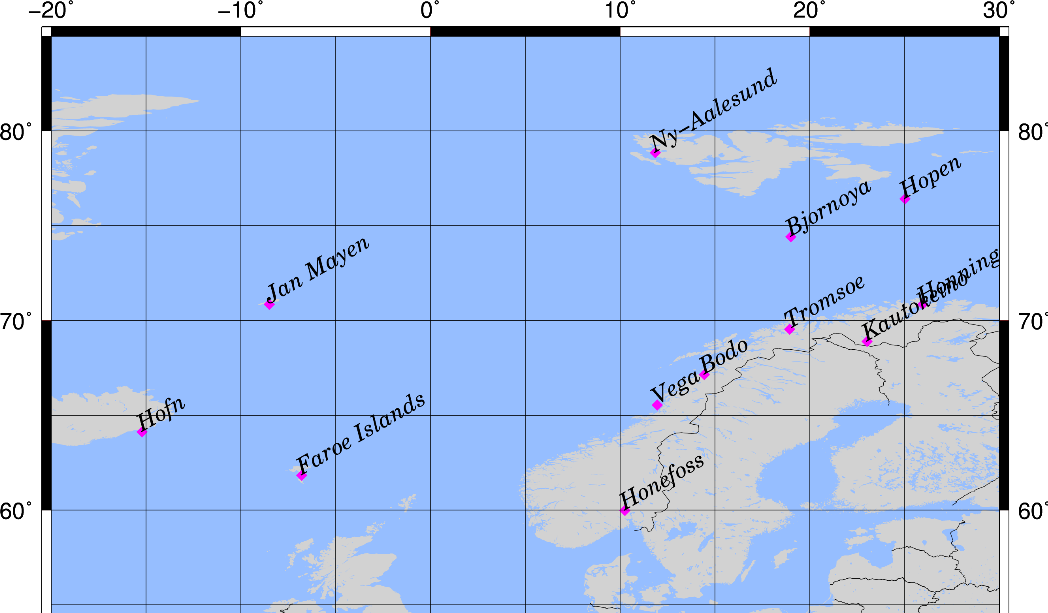
\includegraphics[width=0.7\linewidth]{images/rtisMap}
\end{figure}

\end{frame}

%------------------------------------------------

\begin{frame}
\frametitle{Ionospheric Scintillation}
\begin{itemize}
	\item[] Phenomenon related to solar winds.
	\item[] Randomises electron density.
	\item[] Lessens quality of GNSS observations.
\end{itemize}

\begin{figure}
	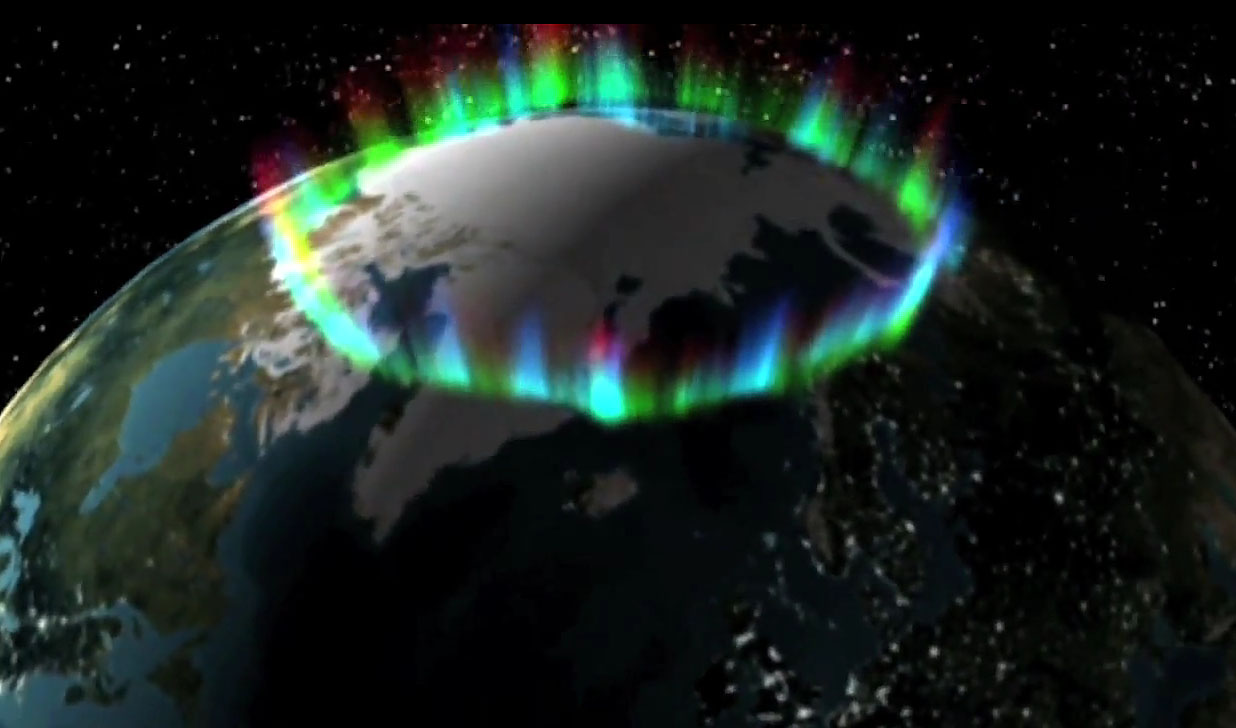
\includegraphics[width=0.7\linewidth]{images/auroral_oval}
\end{figure}

\end{frame}

%------------------------------------------------


\begin{frame}
\frametitle{Goal of the internship}

Create an interface for monitoring the stations:
\begin{itemize}
	\item Visualise data
	\item Get application messages %aka error messages
	\item Change configuration files
	\item Reboot the system
\end{itemize}

\end{frame}

%------------------------------------------------

\section{Architecture}
\frame{\sectionpage}

\begin{frame}
\frametitle{Requirements}
\begin{itemize}
	\item Low bandwidth on some stations
	\begin{itemize}[label=$\Rightarrow$]
		\item Minimise exchanges.
		\item Detect broken connections.
	\end{itemize}
	\item Independent refresh for each type of data.
	\item History of configuration files.
\end{itemize}
\end{frame}

%------------------------------------------------

\begin{frame}
\subsection{First version}
\frametitle{A complex client}
\begin{center}
	\includegraphics[height=0.78\paperheight]{images/global_flowchart_V1}
\end{center}
\end{frame}

\begin{frame}
Problems:
\begin{itemize}
	\item Modifying data sender parameters on the fly.
	\item Detecting disconnects.
	\item[$\Rightarrow$] Complex code.
\end{itemize}

\end{frame}

\subsection{Second version}
\begin{frame}
\frametitle{Too many connections}
\begin{center}
	\includegraphics[height=0.78\paperheight]{images/global_flowchart_V2a}
\end{center}
\end{frame}


\begin{frame}
\frametitle{Too many connections}
\begin{center}
	\includegraphics[height=0.75\paperheight]{images/global_flowchart_V2b}
\end{center}
\end{frame}

\begin{frame}

Problems:
\begin{itemize}
	\item "Blocked-mode" communications
	\begin{itemize}
		\item[$\Rightarrow$] Listening simultaneously on different channels is difficult.
	\end{itemize}
	\item[]
	\item Redundant TCP confirmation for data.
\end{itemize}

\end{frame}

\subsection{Third version}
\begin{frame}
\frametitle{Back to basics.}
\begin{center}
	\includegraphics[height=0.7\paperheight]{images/global_flowchart_V3}
\end{center}
\end{frame}

%------------------------------------------------

\section{Graphical interface}
\frame{\sectionpage}

\subsection{About the configuration files}
\begin{frame}
\frametitle{Storage}
\begin{itemize}
	\item Files stored on the web server
	\begin{itemize}
		\item[$\Rightarrow$] Faster, less bandwidth
		\item[$\Rightarrow$] Keeps track
	\end{itemize}
	\item Simple local database:
	\begin{itemize}
		\item Only one table
		\item Only simple operations (read, write, delete)
	\end{itemize}
\end{itemize}
\end{frame}

\begin{frame}
\frametitle{The web page}

\begin{center}
	\hspace*{-5mm}
	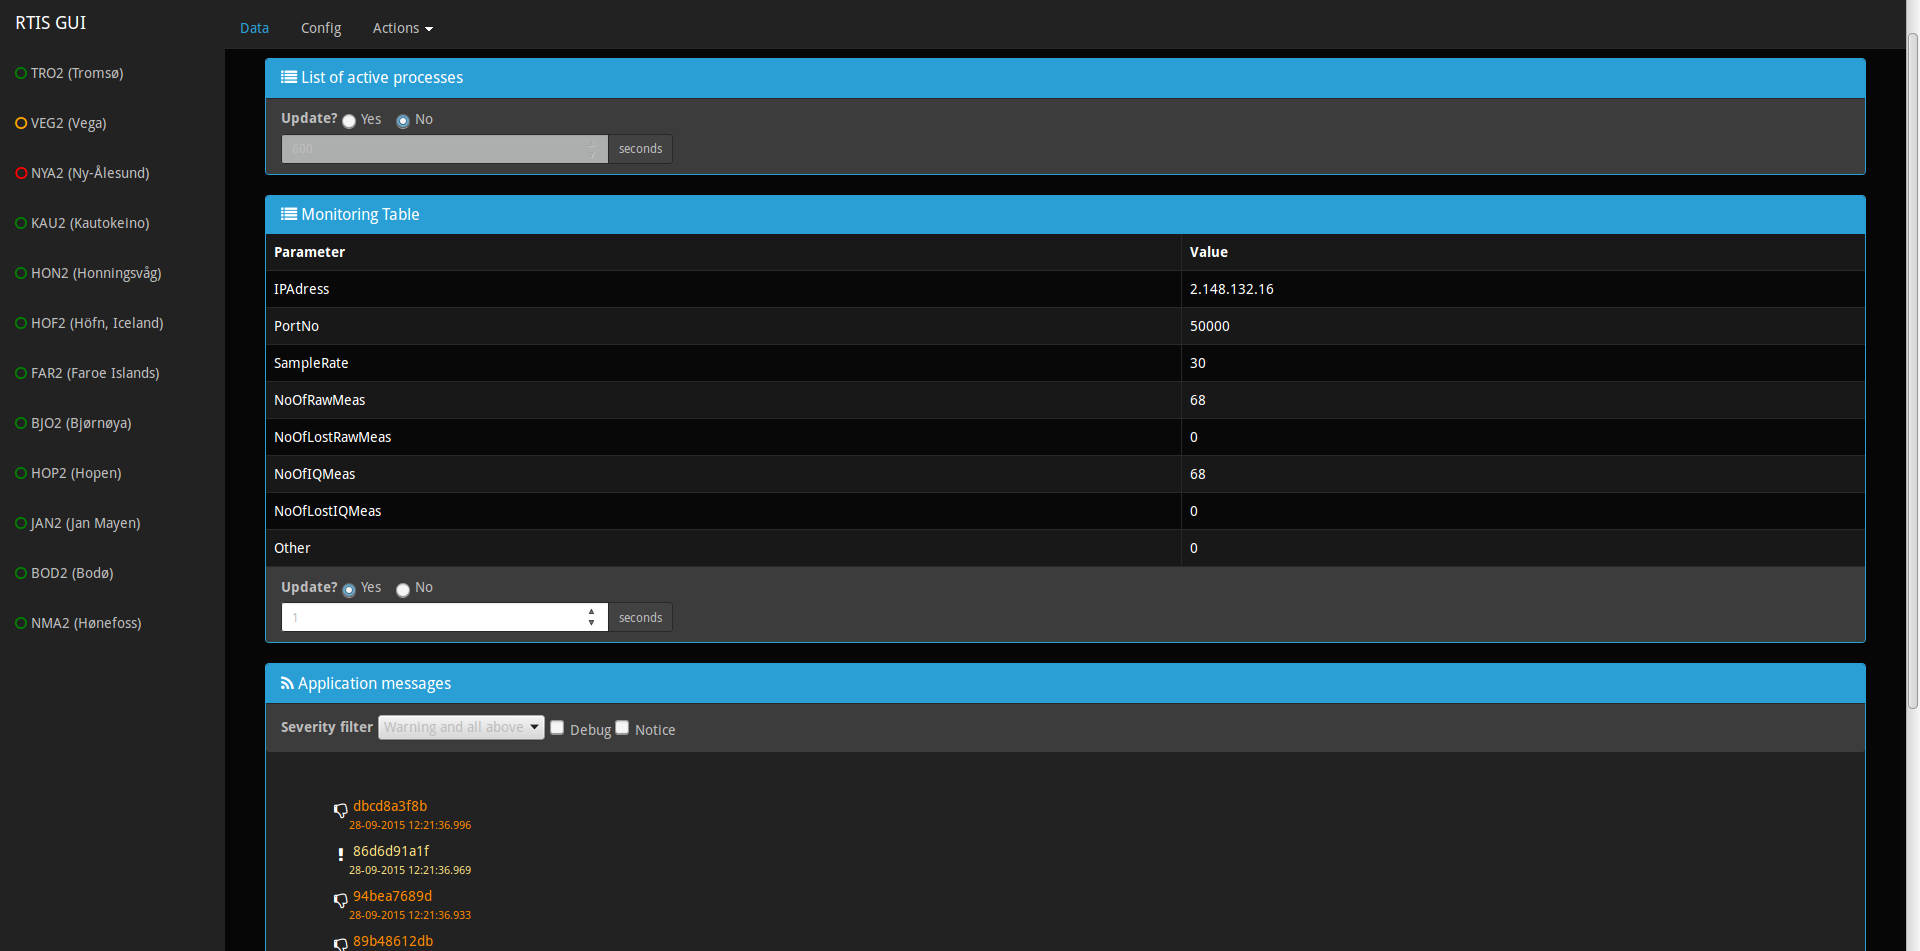
\includegraphics[width=\paperwidth]{images/dataTab}
\end{center}
%PAS LA BONNE IMAGE !\\
%PAS LA BONNE IMAGE !\\
%PAS LA BONNE IMAGE !\\
%PAS LA BONNE IMAGE !\\
%PAS LA BONNE IMAGE !\\
%PAS LA BONNE IMAGE !\\
%PAS LA BONNE IMAGE !\\
%PAS LA BONNE IMAGE !\\
%PAS LA BONNE IMAGE !\\
%PAS LA BONNE IMAGE !\\
%PAS LA BONNE IMAGE !\\
%PAS LA BONNE IMAGE !\\
%PAS LA BONNE IMAGE !\\
%PAS LA BONNE IMAGE !\\

\end{frame}

\subsection{Displaying data}
\begin{frame}
\frametitle{Data tab}
	\hspace*{-5mm}
	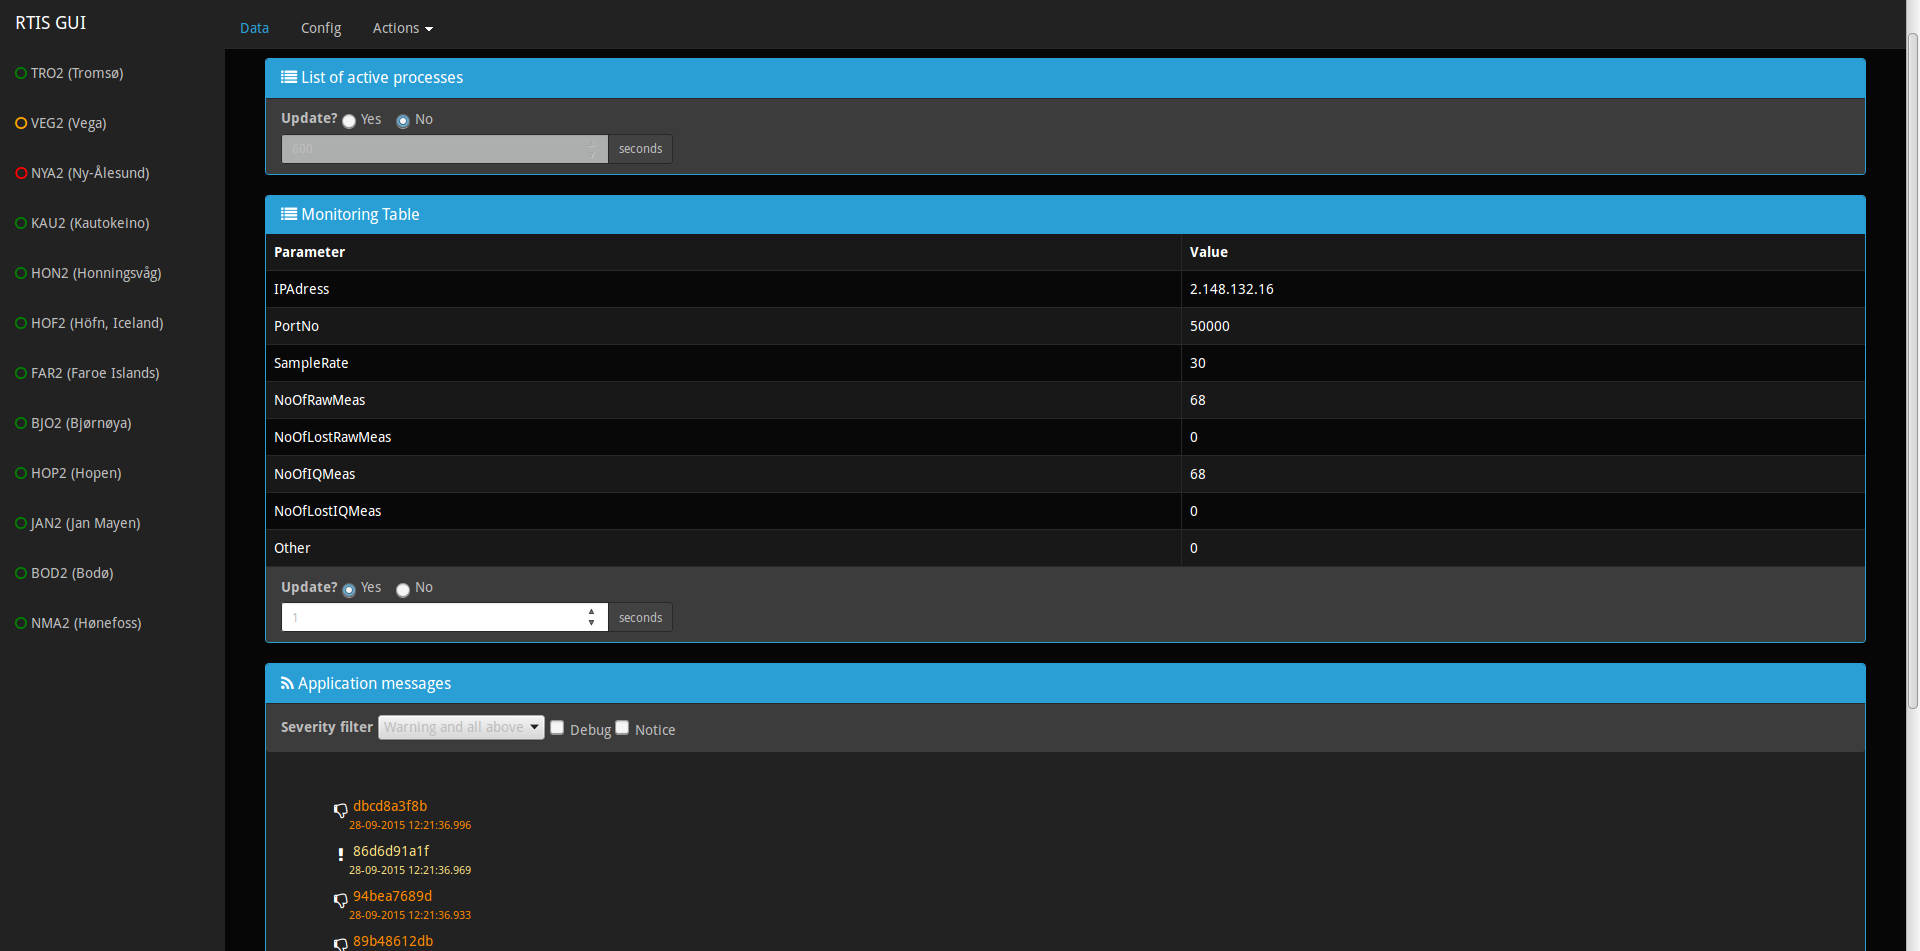
\includegraphics[width=\paperwidth]{images/dataTab}
\end{frame}

%------------------------------------------------
\section{}

\begin{frame}
\Huge{\centerline{The End}}
\end{frame}


%------------------------------------------------
\appendix

{
\setbeamertemplate{footline}
{
  \leavevmode%
  \hbox{%
  \begin{beamercolorbox}[wd=.4\paperwidth,ht=2.25ex,dp=1ex,center]{author in head/foot}%
    \usebeamerfont{author in head/foot}\insertshortauthor
  \end{beamercolorbox}%
  \begin{beamercolorbox}[wd=.6\paperwidth,ht=2.25ex,dp=1ex,center]{title in head/foot}%
    \usebeamerfont{title in head/foot}\insertshorttitle\hspace*{3em}
  \end{beamercolorbox}}%
  \vskip0pt%
}



\begin{frame}[fragile]

\frametitle{C-PHP communications}
\begin{block}{test.c}
	\lstset{language=C}
	\begin{lstlisting}
		main(){
			int x;
			printf("Initialisation");
			x = 1;
			printf("Done");
			return x;
		}
	\end{lstlisting}
\end{block}

\begin{block}{example.php}
	\lstset{language=PHP}
	\begin{lstlisting}
		exec("./test",$output,$returnValue);
		//$output = ["Initialisation","Done"]
		//$returnValue = 1
	\end{lstlisting}
\end{block}

\end{frame}

\bgroup
\setbeamercolor{background canvas}{bg=black}
\begin{frame}[plain]{}
	\hspace*{-4.5mm}
	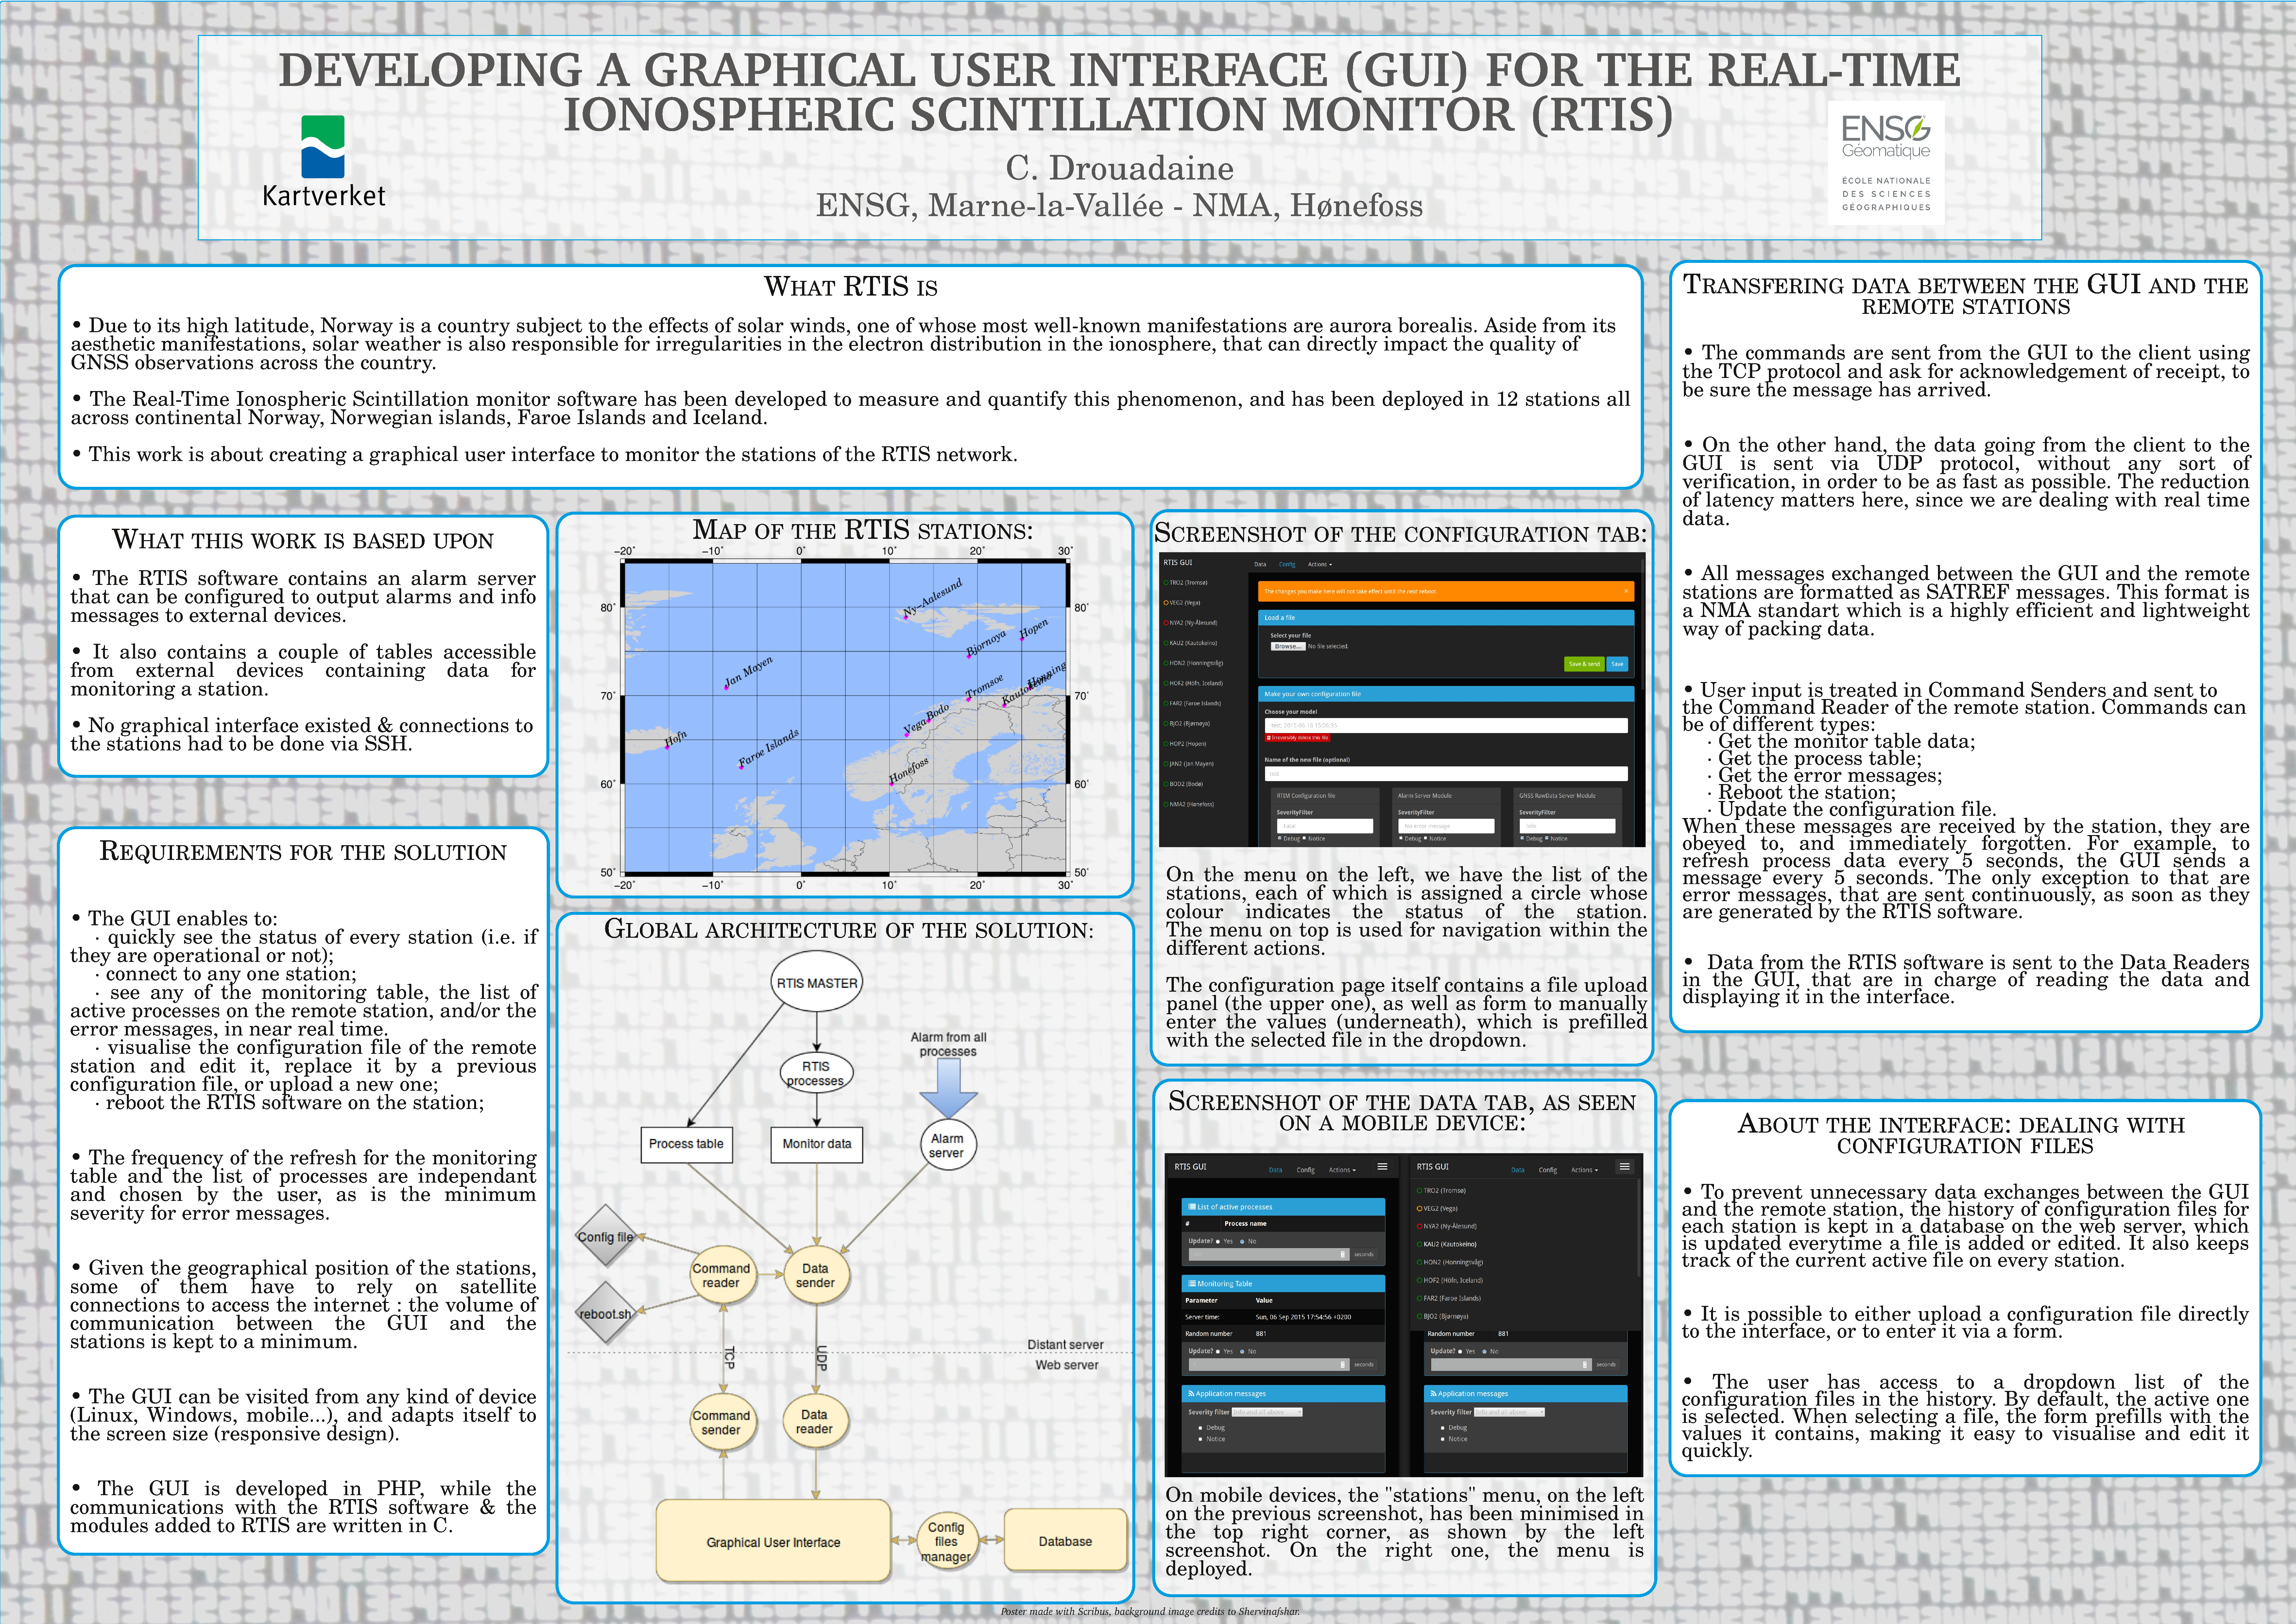
\includegraphics[width=\paperwidth]{../Poster/poster.png}
\end{frame}
\egroup


}

%----------------------------------------------------------------------------------------

\end{document} 